\begin{figure*}[!tp]
  \centering
  \begin{minipage}[t]{\dimexpr.5\textwidth-.5\columnsep\relax}
  \vspace{0pt}
  \centering
  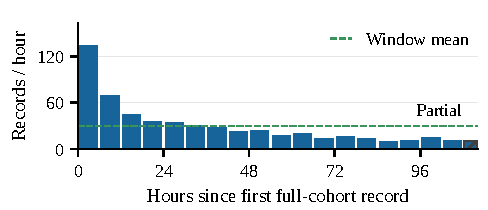
\includegraphics[width=\linewidth,height=1.40in,keepaspectratio]{figures/fig_full_cohort_program_rates.pdf}
  \end{minipage}\hfill
  \begin{minipage}[t]{\dimexpr.5\textwidth-.5\columnsep\relax}
  \vspace{0pt}
  \captionsetup{aboveskip=0pt}
  \caption{\textbf{Full-cohort program-journal rates vary over calendar time.}
  All \num{3364} captured records from rounds 775--4561, through 20:57 UTC
  on 3 November 2026; warm-up records are excluded.
  Eighteen full six-hour bins and one partial bin span the first included
  event to capture. The hatched final bin uses its actual 4.13-hour exposure;
  the dashed line shows mean records per hour. Time includes gaps and waits.
  These recorded-event rates do not measure proposal success, adapter
  admission or learning. Scope: \cref{sec:method-status}.}
  \label{fig:full-cohort-program-rates}
  \end{minipage}
\end{figure*}
